\documentclass[a3paper,12pt]{extarticle} % Use extarticle for A3 paper size
\usepackage{graphicx} % Include this package for \includegraphics
\usepackage{amsmath}
\usepackage{listings}
\usepackage{amssymb} % Include this package for \mathbb
\usepackage[margin=1in]{geometry} % Adjust the margin as needed

\begin{document}

\author{kipngeno koech - bkoech}
\title{Homework 2 - Introduction to Machine Learning for Engineers}
\maketitle

\medskip

\maketitle
\section{Naive Bayes Parameters}
\subsection*{Problem Statement}
The na\"ive Bayes approach assumes that the feature vectors are independent given the label, that is, for any given data point $\mathbf{x}_i = [x_{i1}, x_{i2}, \cdots, x_{id}]^\top$ and its label $y_i$, we have
\[
P(x_{i1}, x_{i2}, \cdots, x_{id}, y_i) = P(y_i) \prod_{j=1}^{d} P(x_{ij} \mid y_i)
\]
Suppose that we are given the data set $\mathbf{X} = [\mathbf{x}_1, \mathbf{x}_2, \cdots, \mathbf{x}_N]^\top$, where $\mathbf{X} \in \mathbb{R}^{N \times 4}$, consisting of $N$ data points and 4 features, and its label $\mathbf{y} = [y_1, y_2, \cdots, y_N]^\top$. Assume that the first feature has 2, the second has 3, the third has 4, and the fourth has 5 possible values: Let $X_1 \in \{1, 2\}$, $X_2 \in \{1, 2, 3\}$, $X_3 \in \{1, 2, 3, 4\}$, and $X_4 \in \{1, 2, 3, 4, 5\}$. Also, there are 4 possible labels, i.e., $Y \in \{1, 2, 3, 4\} \forall i$.

This is what I have:
\[
\text{ Feature 1: } X_1 \in \{1, 2\}
\]
\[
\text{ Feature 2: } X_2 \in \{1, 2, 3\}
\]
\[
\text{ Feature 3: } X_3 \in \{1, 2, 3, 4\}
\]
\[
\text{ Feature 4: } X_4 \in \{1, 2, 3, 4, 5\}
\]
\[
\text{ Label: } Y \in \{1, 2, 3, 4\}
\]
Naive's bayes classifier follow Bayesian rule:
\[
P(Y|X) = \frac{P(X|Y)P(Y)}{P(X)}
\]
Every data point has 4 features and 1 label:
\[
    x_i = [x_{i1}, x_{i2}, x_{i3}, x_{i4}] \quad \text{and} \quad y_i
\]

\begin{enumerate}
    \item[a.] [5 points] Determine the number of free parameters $\theta$ and $\pi$ that one has to estimate using the na\"ive Bayes framework. (We use $\theta$ for the probabilities of a feature given a label (e.g., $\theta_{3,2,4} = P(X_3 = 2 \mid Y = 4)$) and $\pi$ for the class priors (e.g., $\pi_3 = P(Y = 3)$) similar to the lecture slides.)
    \\ Free parameters means those that we need to estimate.
    \\ class priors:
    \[
        \pi_1 = P(Y = 1), \quad \pi_2 = P(Y = 2), \quad \pi_3 = P(Y = 3), \quad \pi_4 = P(Y = 4)
    \]
    We need to estimate only three of these probabilities, since probability always sum up to one. So for class priors we have:
    \[
         \textbf{3}\text{  parameters to estimate}
    \]
    We need to estimate how likely each feature is given a label
    \\ Feature 1: it has 2 possible values, so we need to estimate 2 probabilities for each label
    \[
        \theta_{1,1} = P(X_1 = 1 \mid Y = 1), \quad \theta_{1,2} = P(X_1 = 2 \mid Y = 1)
    \]
    probability should sum up to one, so we only need to estimate one of the probabilities. So for feature 1 given 4 labels, we have:
    \[
        \textbf{4}\text{  parameters to estimate}
    \]
    \\ Feature 2: it has 3 possible values, so we need to estimate 3 probabilities for each label
    \[
        \theta_{2,1} = P(X_2 = 1 \mid Y = 1), \quad \theta_{2,2} = P(X_2 = 2 \mid Y = 1), \quad \theta_{2,3} = P(X_2 = 3 \mid Y = 1)
    \]
    probability should sum up to one, so we only need to estimate two of the probabilities. So for feature 2 given 4 labels, we have:
    \[
        4 \times 2 = \textbf{8}\text{  parameters to estimate}
    \]
    \\ Feature 3: it has 4 possible values, so we need to estimate 4 probabilities for each label:
    \[
        \theta_{3,1} = P(X_3 = 1 \mid Y = 1), \quad \theta_{3,2} = P(X_3 = 2 \mid Y = 1), \quad \theta_{3,3} = P(X_3 = 3 \mid Y = 1), \quad \theta_{3,4} = P(X_3 = 4 \mid Y = 1)
    \]
    probability should sum up to one, so we only need to estimate three of the probabilities. So for feature 3 given 4 labels, we have:
    \[
        4 \times 3 = \textbf{12}\text{  parameters to estimate}
    \]
    \\ Feature 4: it has 5 possible values, so we need to estimate 5 probabilities for each label:
    \[
        \theta_{4,1} = P(X_4 = 1 \mid Y = 1), \quad \theta_{4,2} = P(X_4 = 2 \mid Y = 1), \quad \theta_{4,3} = P(X_4 = 3 \mid Y = 1), \quad \theta_{4,4} = P(X_4 = 4 \mid Y = 1), \quad \theta_{4,5} = P(X_4 = 5 \mid Y = 1)
    \]
    probability should sum up to one, so we only need to estimate four of the probabilities. So for feature 4 given 4 labels, we have:
    \[
        4 \times 4 = \textbf{16}\text{  parameters to estimate}
    \]
    So the total number of parameters to estimate is:
    \[
        3 + 4 + 8 + 12 + 16 = \textbf{43}\text{  parameters to estimate}
    \]

    \item[b.] [4 points] If the features are not independent conditioned on the label, one has to estimate the entire joint distribution $P(X_1, X_2, X_3, X_4 \mid Y = i)$, for all $i \in \{1, 2, 3, 4\}$. Determine the number of free parameters that one has to estimate in such a scenario.
    \\ for each label, we have 4 features, so we need to estimate the entire joint distribution for each label. For each label, we have:
    \\ For each class \(Y = i\):
    \[
        \text{Feature 1: } X_1 \in \{1, 2\}
    \]
    \[
        \text{Feature 2: } X_2 \in \{1, 2, 3\}
    \]
    \[
        \text{Feature 3: } X_3 \in \{1, 2, 3, 4\}
    \]
    \[
        \text{Feature 4: } X_4 \in \{1, 2, 3, 4, 5\}
    \]
    So the total number of possible combinations for each label is:
    \[
        2 \times 3 \times 4 \times 5 = 120
    \]
    When we add the joint distribution for every label, it should sum up to one. So the total number of parameters to estimate is:
    \[
    120 - 1 = \textbf{119}\text{  parameters to estimate}
    \]
    We have 4 labels, so the total number of parameters to estimate is:
    \[
    4 \times 119 = \textbf{476}\text{  parameters to estimate}
    \]
    \item[c.] [1 point] Based on the numbers of parameters you found in parts (a) and (b), explain one advantage of assuming conditional independence.
    \\ The advantage of assuming conditional independence is that it reduces the number of parameters that we need to estimate. This makes the model less complex and easier to train. It also reduces the risk of overfitting the model.
\end{enumerate}
\newpage
\section{Naive Bayes in Practice}

In this problem we will use the na\"ive Bayes algorithm to classify movie reviews as positive, neutral or negative. A simple approach involves maintaining a vocabulary of words that commonly occur in movie reviews and using the frequency of their occurrence in the three classes to classify movie reviews.

We are given the vocabulary $V = \{ 1:\text{``incredible''}, 2:\text{``plot''}, 3:\text{``great''}, 4:\text{``amazing''}, 5:\text{``okay''}, 6:\text{``decent''}, 7:\text{``movie''}, 8:\text{``no''}, 9:\text{``acting''}, 10:\text{``waste''} \}$. We will use $V_i$ to represent the $i$th word in $V$. The training set provided includes four positive reviews:
\begin{itemize}
    \item ``great movie amazing''
    \item ``incredible movie''
    \item ``great acting amazing plot''
    \item ``amazing acting amazing plot''
\end{itemize}
two neutral reviews:
\begin{itemize}
    \item ``okay movie''
    \item ``decent no amazing acting''
\end{itemize}
and two negative reviews:
\begin{itemize}
    \item ``amazing waste''
    \item ``no movie plot''
\end{itemize}

Recall that the na\"ive Bayes classifier is a generative classifier, where the probability of an input $\mathbf{x} = [x_1, x_2, \cdots, x_n]^\top$ depends on its class $y$. In our case the input vector $\mathbf{x}$ corresponding to each movie review has $n = 10$ equal to the number of words in the vocabulary $V$, where each entry $x_i$ is equal to the number of times word $V_i$ occurs in $\mathbf{x}$.
\[\]
Understanding the problem at hand:

We have three classes:

1. Positive reviews: ``great movie amazing'', ``incredible movie'', ``great acting amazing plot'', ``amazing acting amazing plot''

2. Neutral reviews: ``okay movie'', ``decent no amazing acting''

3. Negative reviews: ``amazing waste'', ``no movie plot''
\[ \\
\]
We have a vocabulary of 10 words:

1. ``incredible''

2. ``plot''

3. ``great''

4. ``amazing''

5. ``okay''

6. ``decent''

7. ``movie''

8. ``no''

9. ``acting''

10. ``waste''

\[\]
Encoding the reviews - We encode the reviews as feature vectors, where each entry in the vector corresponds to the number of times a word in the vocabulary appears in the review:
\\ Positive reviews:
\[
\text{``great movie amazing''} \rightarrow [0, 0, 1, 1, 0, 0, 1, 0, 0, 0]
\]
\[
\text{``incredible movie''} \rightarrow [1, 0, 0, 0, 0, 0, 1, 0, 0, 0]
\]
\[
\text{``great acting amazing plot''} \rightarrow [0, 1, 1, 1, 0, 0, 0, 0, 1, 0]
\]
\[
\text{``amazing acting amazing plot''} \rightarrow [0, 1, 0, 2, 0, 0, 0, 0, 1, 0]
\]
Neutral reviews:
\[
\text{``okay movie''} \rightarrow [0, 0, 0, 0, 1, 0, 1, 0, 0, 0]
\]
\[
\text{``decent no amazing acting''} \rightarrow [0, 0, 0, 1, 0, 1, 0, 1, 1, 0]
\]
Negative reviews:
\[
\text{``amazing waste''} \rightarrow [0, 0, 0, 1, 0, 0, 0, 0, 0, 1]
\]
\[
\text{``no movie plot''} \rightarrow [0, 1, 0, 0, 0, 0, 1, 1, 0, 0]
\]

\begin{enumerate}
    \item[a.] [2 points] Calculate the na\"ive Bayes estimates of $\Pr(y = 1)$, $\Pr(y = 2)$ and $\Pr(y = 3)$ from the training data, where $y = 1$ corresponds to positive reviews, $y = 2$ to neutral reviews and $y = 3$ to negative reviews.
    \\ We have 4 positive reviews, 2 neutral reviews and 2 negative reviews. So the prior probabilities are:
    \[
        \Pr(y) = \frac{\text{number of reviews of class } y}{\text{total number of reviews}}
    \]
    \[
    \Pr(y = 1) = \frac{4}{8} = \frac{1}{2}
    \]
    \[
    \Pr(y = 2) = \frac{2}{8} = \frac{1}{4}
    \]
    \[
    \Pr(y = 3) = \frac{2}{8} = \frac{1}{4}
    \]
    \item[b.] [1 point] List the feature vector $\mathbf{x}$ for each positive review in the training set.
    \[
    \text{``great movie amazing''} \rightarrow [0, 0, 1, 1, 0, 0, 1, 0, 0, 0]
    \]
    \[
    \text{``incredible movie''} \rightarrow [1, 0, 0, 0, 0, 0, 1, 0, 0, 0]
    \]
    \[
    \text{``great acting amazing plot''} \rightarrow [0, 1, 1, 1, 0, 0, 0, 0, 1, 0]
    \]
    \item[c.] [2 points] In the na\"ive Bayes model, the likelihood of a sentence with feature vector $\mathbf{x}$ given a class $c$ is
    \[
    \Pr(\mathbf{x} \mid y = c) = \prod_{k=1}^{n} (\theta_{c,k})^{x_k}
    \]
    where $\theta_{c,k}$ is the weight of word $k$ among all words of class $c$. Calculate the maximum likelihood estimate of $\theta_{1,4}$, $\theta_{1,7}$, $\theta_{2,4}$, $\theta_{2,7}$, $\theta_{3,4}$ and $\theta_{3,7}$.
    \\ For each class, we need to estimate the probability of each word given the class. We can calculate the maximum likelihood estimate of $\theta_{c,k}$ as:
    \[
    \theta_{c,k} = \frac{\text{number of times word } k \text{ appears in class } c}{\text{total number of words in class } c}
    \]
    For class 1 (positive reviews):
    \[
    \theta_{1,4} = \theta_{\text{positive}, \text{amazing}} = \frac{4}{13} = \frac{4}{13}
    \]
    \[
    \theta_{1,7} = \theta_{\text{positive}, \text{movie}} = \frac{2}{13} = \frac{2}{13}
    \]
    For class 2 (neutral reviews):
    \[
    \theta_{2,4} = \theta_{\text{neutral}, \text{amazing}} = \frac{1}{6} = \frac{1}{6}
    \]
    \[
    \theta_{2,7} = \theta_{\text{neutral}, \text{movie}} = \frac{1}{6} = \frac{1}{6}
    \]
    For class 3 (negative reviews):
    \[
    \theta_{3,4} = \theta_{\text{negative}, \text{amazing}} = \frac{1}{5} = \frac{1}{5}
    \]
    \[
    \theta_{3,7} = \theta_{\text{negative}, \text{movie}} = \frac{1}{5} = \frac{1}{5}
    \]
    \item[d.] [3 points] Given a new review ``amazing movie'', decide whether it is positive, neutral or negative, based on the na\"ive Bayes classifier, learned from the above data.
    \[
    \Pr(y = c \mid \mathbf{x}) \propto \Pr(\mathbf{x} \mid y = c) \Pr(y = c)
    \]
    For the new review ``amazing movie'', the feature vector is:
    \[
    \mathbf{x} = [0, 0, 0, 1, 0, 0, 1, 0, 0, 0]
    \]
    We can calculate the probability of the review being positive, neutral or negative as:
    \[
        \Pr(\text{class} \mid \text{word} ) = \Pr(\text{word} \mid \text{class}) \Pr(\text{class})
    \]
    We can calculate the probabilities as:
    \\ class positive:
    \[
    \Pr(\text{positive} \mid \text{word} ) = \theta_{1,4}^{1} \times \theta_{1,7}^{1} \times \Pr(\text{positive})
    \]
    \[
    \Pr(\text{positive} \mid \text{word} ) = \left( \frac{4}{13} \right) \times \left( \frac{2}{13} \right) \times \frac{1}{2} = \frac{8}{338}
    \]
    \\ class neutral:
    \[
    \Pr(\text{neutral} \mid \text{word} ) = \theta_{2,4}^{1} \times \theta_{2,7}^{1} \times \Pr(\text{neutral})
    \]
    \[
    \Pr(\text{neutral} \mid \text{word} ) = \left( \frac{1}{6} \right) \times \left( \frac{1}{6} \right) \times \frac{1}{4} = \frac{1}{144}
    \]
    \\ class negative:
    \[
    \Pr(\text{negative} \mid \text{word} ) = \theta_{3,4}^{1} \times \theta_{3,7}^{1} \times \Pr(\text{negative})
    \]
    \[
    \Pr(\text{negative} \mid \text{word} ) = \left( \frac{1}{5} \right) \times \left( \frac{1}{5} \right) \times \frac{1}{4} = \frac{1}{100}
    \]

    \item[e.] [4 points] Use Laplacian smoothing with $\alpha = 1$ to decide whether the review ``decent movie'' is positive, neutral or negative. In one sentence, describe the problem we would encounter if we had not used Laplacian smoothing.
    \\ Laplacian smoothing is used to avoid zero probabilities. We add a small value to the numerator and denominator to avoid zero probabilities. The probability of a word given a class is calculated as:
    \[
    \theta_{c,k} = \frac{\text{number of times word } k \text{ appears in class } c + \alpha}{\text{total number of words in class } c + \alpha \times \text{number of words in the vocabulary}}
    \]
    For the new review ``decent movie'', the feature vector is:
    \[
    \mathbf{x} = [0, 0, 0, 0, 0, 1, 1, 0, 0, 0]
    \]
    We can calculate the probability of the review being positive, neutral or negative as:
    \\ class positive:
    \[
    \Pr(\text{positive} \mid \text{word} ) = \theta_{1,6}^{1} \times \theta_{1,7}^{1} \times \Pr(\text{positive})
    \]
    \[
    \Pr(\text{positive} \mid \text{word} ) = \left( \frac{1}{13} \right) \times \left( \frac{2}{13} \right) \times \frac{1}{2} = \frac{2}{338}
    \]
    \\ class neutral:
    \[
    \Pr(\text{neutral} \mid \text{word} ) = \theta_{2,6}^{1} \times \theta_{2,7}^{1} \times \Pr(\text{neutral})
    \]
    \[
    \Pr(\text{neutral} \mid \text{word} ) = \left( \frac{2}{6} \right) \times \left( \frac{1}{6} \right) \times \frac{1}{4} = \frac{1}{72}
    \]
    \\ class negative:
    \[
    \Pr(\text{negative} \mid \text{word} ) = \theta_{3,6}^{1} \times \theta_{3,7}^{1} \times \Pr(\text{negative})
    \]
    \[
    \Pr(\text{negative} \mid \text{word} ) = \left( \frac{1}{5} \right) \times \left( \frac{1}{5} \right) \times \frac{1}{4} = \frac{1}{100}
    \]
    If we had not used Laplacian smoothing, we would have encountered zero probabilities, which would have made it impossible to calculate the probabilities.
\end{enumerate}
\newpage
\section{Logistic Regression in Practice}
Given a training set \( D = \left\{ \left( \mathbf{x}^{(1)}, y^{(1)} \right), \dots, \left( \mathbf{x}^{(N)}, y^{(N)} \right) \right\} \) where \( \left( \mathbf{x}^{(i)} \in \mathbb{R}^d, y^{(i)} \in \{0, 1\} \right) \) is the feature vector and the binary label for data point \( i \), we want to find the parameters \( \hat{\mathbf{w}} \) that maximize the likelihood for the training set, assuming a parametric model of the form
\[
p(y = 1 \mid \mathbf{x}, \mathbf{w}) = \frac{1}{1 + \exp(-\mathbf{w}^T \mathbf{x})}.
\]
The conditional log likelihood of the training set is
\[
L(\mathbf{w}) = \sum_{i=1}^N \left[ y^{(i)} \log p\left( y^{(i)} \mid \mathbf{x}^{(i)}, \mathbf{w} \right) + \left( 1 - y^{(i)} \right) \log \left( 1 - p\left( y^{(i)} \mid \mathbf{x}^{(i)}, \mathbf{w} \right) \right) \right],
\]
and the gradient is
\[
\nabla L(\mathbf{w}) = \sum_{i=1}^N \left( y^{(i)} - p\left( y^{(i)} \mid \mathbf{x}^{(i)}, \mathbf{w} \right) \right) \mathbf{x}^{(i)}. \quad (2)
\]

\noindent \textbf{a.} [2 points] Is it possible to get a closed form for the parameters \( \hat{\mathbf{w}} \) that maximize the conditional log likelihood? If it is possible, give the closed-form solution. If not, how would you compute \( \hat{\mathbf{w}} \) in practice? Explain your method to find \( \hat{\mathbf{w}} \) in a few sentences or provide a short pseudo-code.
\\\\ It is not possible to get a closed form for the parameters \( \hat{\mathbf{w}} \) that maximize the conditional log likelihood. We can use gradient descent to find the parameters \( \hat{\mathbf{w}} \). The gradient of the conditional log likelihood is given by Eq. (2). We can update the parameters \( \mathbf{w} \) using the update rule:
\[
\mathbf{w}_{(k+1)} = \mathbf{w}_{(k)} + \alpha \nabla L(\mathbf{w}_{(k)}),
\]
The  pseudo-code to find the parameters \( \hat{\mathbf{w}} \) is as follows:
\begin{lstlisting}
    Initialize w
    while not converged:
        for i in range(N):
            w = w + alpha * gradL(w)
\end{lstlisting}
where \( \alpha \) is the learning rate, \( N \) is the number of data points, and \( \text{gradL}(\mathbf{w}) \) is the gradient of the conditional log likelihood.\\


For a binary logistic regression model, we predict \( y = 1 \) when \( p(y = 1 \mid \mathbf{x}) \geq 0.5 \). Assume that the decision boundary occurs when \( P(y = 1 \mid \mathbf{x}, \mathbf{w}) = P(y = 0 \mid \mathbf{x}, \mathbf{w}) \).

\noindent \textbf{b.} [4 points] Find the decision boundary, which is the set of $\mathbf{x}$ satisfying $P(y = 1 \mid \mathbf{x}, \mathbf{w}) = P(y = 0 \mid \mathbf{x}, \mathbf{w})$.

we have:
\[
P(y = 1 \mid \mathbf{x}, \mathbf{w}) = P(y = 0 \mid \mathbf{x}, \mathbf{w})
\]
\[
\frac{1}{1 + \exp(-\mathbf{w}^T \mathbf{x})} = 1 - \frac{1}{1 + \exp(-\mathbf{w}^T \mathbf{x})}
\]
\[
\frac{1}{1 + \exp(-\mathbf{w}^T \mathbf{x})} = \frac{1 + \exp(-\mathbf{w}^T \mathbf{x}) - 1}{1 + \exp(-\mathbf{w}^T \mathbf{x})}
\]
\[
\frac{1}{1 + \exp(-\mathbf{w}^T \mathbf{x})} = \frac{\exp(-\mathbf{w}^T \mathbf{x})}{1 + \exp(-\mathbf{w}^T \mathbf{x})}
\]
\[
1 = \exp(-\mathbf{w}^T \mathbf{x})
\]
\[
\log(1) = \log(\exp(-\mathbf{w}^T \mathbf{x}))
\]
\[
0 = -\mathbf{w}^T \mathbf{x}
\]
\[
\mathbf{w}^T \mathbf{x} = 0
\]
The decision boundary is given by the equation \( \mathbf{w}^T \mathbf{x} = 0 \).

\noindent \textbf{c.} [1 point] Is this model a linear classifier?
\\\\yes, this model is a linear classifier. The decision boundary is a linear function of the input features \( \mathbf{x} \) and the model predicts the class based on whether the input lies above or below this linear boundary.\\

\noindent \textbf{d.} [2 points] Now, let us assume that in our application of this model, our tolerance of mis-classifying samples with the true label $y = 0$ is much lower than our tolerance to mis-classifying samples with true label $y = 1$ (i.e., we do not want to estimate a data point as belonging to class 0 if its true class is 1. However, we can tolerate the error of estimating a data point belong to class 1 if its true class is 0.) For example, in predicting the presence of a disease, we may be much more tolerant of mis-classifying a healthy person (true label $y = 0$) as having the disease ($y = 1$) compared to mis-classifying a person with the disease (true label $y = 1$) as not having it ($y = 0$). Now suppose you have trained a logistic regression model to obtain the model weights $\mathbf{w}$. How would you adjust the prediction with weights $\mathbf{w}$ to decrease the mis-classification of samples with true label $y = 1$?
\\\\We  can adjust the prediction threshold to decrease the mis-classification of samples with true label \( y = 1 \). We can increase the threshold to predict \( y = 1 \) only when the probability is higher than the threshold. This will decrease the number of false positives. We can adjust the threshold to increase the number of true positives and decrease the number of false positives.\\
 
\newpage
\section{Solving Logistic Regression}
The cross-entropy loss function for a logistic regression task on a dataset \( \{(\mathbf{x}_1, y_1), (\mathbf{x}_2, y_2), \dots, (\mathbf{x}_n, y_n)\} \) can be written as
\[
L(\mathbf{w}) = -\sum_{i=1}^n \left[ y_i \log p(y_i \mid \mathbf{x}_i, \mathbf{w}) + (1 - y_i) \log (1 - p(y_i \mid \mathbf{x}_i, \mathbf{w})) \right],
\]
In this question, we will show that finding the MLE (maximum likelihood estimator) is equivalent to minimizing the cross-entropy loss in Eq. (3). However, unlike linear regression, it is difficult to derive a closed-form solution for logistic regression.

\[
\textbf{a.} \quad [3 points] \quad \text{Starting from the definition of negative log-likelihood (Eq. (4) below), show that it is equal to the cross-entropy loss (Eq. (3)).}
\]

% The negative log-likelihood is given by:
\[
-\ell(\mathbf{w}) = -\log \left( \prod_{i=1}^n \left( \frac{1}{1 + \exp(-\mathbf{w}^\top \mathbf{x}_i)} \right)^{y_i} \left( 1 - \frac{1}{1 + \exp(-\mathbf{w}^\top \mathbf{x}_i)} \right)^{1 - y_i} \right). \quad (4)
\]

% Show that this is equivalent to the cross-entropy loss:
% \[
% L(\mathbf{w}) = -\sum_{i=1}^n \left[ y_i \log \left( \frac{1}{1 + \exp(-\mathbf{w}^\top \mathbf{x}_i)} \right) + (1 - y_i) \log \left( 1 - \frac{1}{1 + \exp(-\mathbf{w}^\top \mathbf{x}_i)} \right) \right]. \quad (3)
% \]

To show that Eq. (4) is equivalent to Eq. (3), We need to expand the terms in Eq. (4) and simplifying the expression:
\[
-\ell(\mathbf{w}) = -\log \left( \prod_{i=1}^n \left( \frac{1}{1 + \exp(-\mathbf{w}^\top \mathbf{x}_i)} \right)^{y_i} \left( 1 - \frac{1}{1 + \exp(-\mathbf{w}^\top \mathbf{x}_i)} \right)^{1 - y_i} \right)
\]
\[
-\ell(\mathbf{w}) = -\sum_{i=1}^n \log \left( \left( \frac{1}{1 + \exp(-\mathbf{w}^\top \mathbf{x}_i)} \right)^{y_i} \left( 1 - \frac{1}{1 + \exp(-\mathbf{w}^\top \mathbf{x}_i)} \right)^{1 - y_i} \right)
\]
\[
-\ell(\mathbf{w}) = -\sum_{i=1}^n \log \left( \left( \frac{1}{1 + \exp(-\mathbf{w}^\top \mathbf{x}_i)} \right)^{y_i} \left( 1 - \frac{1}{1 + \exp(-\mathbf{w}^\top \mathbf{x}_i)} \right)^{1 - y_i} \right)
\]
\[
-\ell(\mathbf{w}) = -\sum_{i=1}^n \log \left( \frac{1}{1 + \exp(-\mathbf{w}^\top \mathbf{x}_i)} \right)^{y_i} \log \left( 1 - \frac{1}{1 + \exp(-\mathbf{w}^\top \mathbf{x}_i)} \right)^{1 - y_i}
\]
\[
-\ell(\mathbf{w}) = -\sum_{i=1}^n y_i \log \left( \frac{1}{1 + \exp(-\mathbf{w}^\top \mathbf{x}_i)} \right) + (1 - y_i) \log \left( 1 - \frac{1}{1 + \exp(-\mathbf{w}^\top \mathbf{x}_i)}\right)
\]
\[
-\ell(\mathbf{w}) = -\sum_{i=1}^n y_i \log \left( \frac{1}{1 + \exp(-\mathbf{w}^\top \mathbf{x}_i)} \right) + (1 - y_i) \log \left( 1 - \frac{1}{1 + \exp(-\mathbf{w}^\top \mathbf{x}_i)} \right)
\]
\[
-\ell(\mathbf{w}) = -\sum_{i=1}^n y_i \log \left( \frac{1}{1 + \exp(-\mathbf{w}^\top \mathbf{x}_i)} \right) + (1 - y_i) \log \left( 1 - \frac{1}{1 + \exp(-\mathbf{w}^\top \mathbf{x}_i)} \right)
\]
let:
\[
p(y_i \mid \mathbf{x}_i, \mathbf{w}) = \frac{1}{1 + \exp(-\mathbf{w}^\top \mathbf{x}_i)}
\]
so we have:
\[
-\ell(\mathbf{w}) = -\sum_{i=1}^n y_i \log p(y_i \mid \mathbf{x}_i, \mathbf{w}) + (1 - y_i) \log (1 - p(y_i \mid \mathbf{x}_i, \mathbf{w}))
\]
\[
-\ell(\mathbf{w}) = L(\mathbf{w})
\]

\textbf{b.} [4 points] Since it is difficult to directly optimize Eq. (3), gradient descent algorithms are usually used to find the optimum, as is discussed in the lecture. Show that the negative log-likelihood is a convex function. You may use the facts that the sum of convex functions is also convex, and that if $f$ and $g$ are both convex, twice differentiable and $g$ is non-decreasing, then $g(f)$ is convex.

\textit{Hint}: A function $f$ is convex if for any $x_1, x_2 \in \text{Domain}(f)$,
\[
f(tx_1 + (1 - t)x_2) \leq t f(x_1) + (1 - t) f(x_2), \quad \forall t \in [0, 1] \quad (5)
\]
Also, a twice-differentiable function is convex if and only if the Hessian is positive semi-definite.
\[
\text{Hessian} = \begin{bmatrix}
    \frac{\partial^2 f}{\partial x_1^2} & \frac{\partial^2 f}{\partial x_1 \partial x_2} & \cdots & \frac{\partial^2 f}{\partial x_1 \partial x_n} \\
    \frac{\partial^2 f}{\partial x_2 \partial x_1} & \frac{\partial^2 f}{\partial x_2^2} & \cdots & \frac{\partial^2 f}{\partial x_2 \partial x_n} \\
    \vdots & \vdots & \ddots & \vdots \\
    \frac{\partial^2 f}{\partial x_n \partial x_1} & \frac{\partial^2 f}{\partial x_n \partial x_2} & \cdots & \frac{\partial^2 f}{\partial x_n^2}
\end{bmatrix}
\]
We can show that the negative log-likelihood is a convex function by showing that the Hessian is positive semi-definite. The Hessian of the negative log-likelihood is given by:
\\ The equation we want to find derivative of is:
\[
-\ell(\mathbf{w}) = -\sum_{i=1}^n y_i \log p(y_i \mid \mathbf{x}_i, \mathbf{w}) + (1 - y_i) \log (1 - p(y_i \mid \mathbf{x}_i, \mathbf{w}))
\]
Let \(P(y_i \mid \mathbf{x}_i, \mathbf{w}) = p\), then the negative log-likelihood is:
\[
-\ell(\mathbf{w}) = -\sum_{i=1}^n y_i \log p + (1 - y_i) \log (1 - p)
\]
The gradient of the negative log-likelihood is:
\[
\nabla \ell(\mathbf{w}) = \sum_{i=1}^n \left( p - y_i \right) \mathbf{x}_i
\]
This is because the derivative of \( \log p \) is \( \frac{1}{p} \) and the derivative of \( \log (1 - p) \) is \( \frac{-1}{1 - p} \). 
\\ The Hessian of the negative log-likelihood is:
\[
\nabla^2 \ell(\mathbf{w}) = \sum_{i=1}^n p(1 - p) \mathbf{x}_i \mathbf{x}_i^T
\]
The Hessian is positive semi-definite because \( p(1 - p) \geq 0 \) and \( \mathbf{x}_i \mathbf{x}_i^T \) is positive semi-definite. Therefore, the negative log-likelihood is a convex function.\\

We now turn our attention to another algorithm known as iterative weighted least squares, which is based on the Newton-Raphson algorithm. Let $\mathbf{w}^{(k)}$ denote the parameter vector $\mathbf{w}$ at the $k$th iteration. Then, the update rule of iterative weighted least-squares is as follows:
\[
\mathbf{w}_{(k+1)} = \mathbf{w}_{(k)} - \left( \nabla^2\mathcal{L}\mathbf{w}_{(k)} \right)^{-1} \nabla L(\mathbf{w}_{(k)}),
\]
where \( \nabla L(\mathbf{w}) \) and \( \nabla^2 L(\mathbf{w}) \) are the gradient and Hessian of the negative log-likelihood in Eq. (3), respectively. Consider the following notations:
\begin{itemize}
    \item \( \mathbf{y} \) is an \( N \times 1 \) column vector with the \( i \)-th element being the label \( y_i \),
    \item \( \mathbf{X} \) is an \( N \times d \) matrix with \( \mathbf{x}_i^\top \) being the \( i \)-th row,
    \item \( \mathbf{W}_k \) is an \( N \times N \) diagonal matrix with the \( i \)-th diagonal element being \( \frac{\exp(-\mathbf{w}_k^\top \mathbf{x}_i)}{(1 + \exp(-\mathbf{w}_k^\top \mathbf{x}_i))^2} \),
    \item \( \mathbf{p}_k \) is an \( N \times 1 \) column vector with the \( i \)-th element being \( \frac{1}{1 + \exp(-\mathbf{w}_k^\top \mathbf{x}_i)} \),
    \item \( \mathbf{z}_k = \mathbf{X} \mathbf{w}_k + \mathbf{W}_k^{-1} (\mathbf{y} - \mathbf{p}_k) \).
\end{itemize}

It can be shown that:
\begin{itemize}
    \item \( \nabla L(\mathbf{w}_k) = -\mathbf{X}^\top (\mathbf{y} - \mathbf{p}_k) \),
    \item \( \nabla^2 L(\mathbf{w}_k) = \mathbf{X}^\top \mathbf{W}_k \mathbf{X} \).
\end{itemize}

\textbf{ c }[5 points] Using the above, prove that
\[
\mathbf{w}_{k+1} = (\mathbf{X}^\top \mathbf{W}_k \mathbf{X})^{-1} \mathbf{X}^\top \mathbf{W}_k \mathbf{z}_k.
\]

Note: The name of the algorithm comes from the observation that the algorithm at each step is solving the weighted least squares problem,
\[
\mathbf{w}_{k+1} = \arg\min_{\mathbf{w}_k} (\mathbf{z}_k - \mathbf{X} \mathbf{w}_k)^\top \mathbf{W}_k (\mathbf{z}_k - \mathbf{X} \mathbf{w}_k).
\]

To prove the equation, we need to show that:
\[
\mathbf{w}_{k+1} = (\mathbf{X}^\top \mathbf{W}_k \mathbf{X})^{-1} \mathbf{X}^\top \mathbf{W}_k \mathbf{z}_k
\]
We have:
\[
\mathbf{w}_{k+1} = \mathbf{w}_k - \left( \nabla^2\mathcal{L}\mathbf{w}_k \right)^{-1} \nabla L(\mathbf{w}_k)
\]
We know that:
\[
\nabla L(\mathbf{w}_k) = -\mathbf{X}^\top (\mathbf{y} - \mathbf{p}_k)
\]
\[
\nabla^2 L(\mathbf{w}_k) = \mathbf{X}^\top \mathbf{W}_k \mathbf{X}
\]
Substituting the values of \( \nabla L(\mathbf{w}_k) \) and \( \nabla^2 L(\mathbf{w}_k) \) into the update rule, we get:
\[
\mathbf{w}_{k+1} = \mathbf{w}_k - \left( \mathbf{X}^\top \mathbf{W}_k \mathbf{X} \right)^{-1} \left( -\mathbf{X}^\top (\mathbf{y} - \mathbf{p}_k) \right)
\]
\[
\mathbf{w}_{k+1} = \mathbf{w}_k + \left( \mathbf{X}^\top \mathbf{W}_k \mathbf{X} \right)^{-1} \mathbf{X}^\top (\mathbf{y} - \mathbf{p}_k)
\]
\[
\mathbf{w}_{k+1} = \mathbf{w}_k + \left( \mathbf{X}^\top \mathbf{W}_k \mathbf{X} \right)^{-1} \mathbf{X}^\top \mathbf{W}_k \mathbf{X} \mathbf{w}_k - \left( \mathbf{X}^\top \mathbf{W}_k \mathbf{X} \right)^{-1} \mathbf{X}^\top \mathbf{W}_k \mathbf{y}
\]
\[
\mathbf{w}_{k+1} = \left( \mathbf{X}^\top \mathbf{W}_k \mathbf{X} \right)^{-1} \mathbf{X}^\top \mathbf{W}_k \mathbf{X} \mathbf{w}_k + \left( \mathbf{X}^\top \mathbf{W}_k \mathbf{X} \right)^{-1} \mathbf{X}^\top \mathbf{W}_k \mathbf{X} \mathbf{w}_k - \left( \mathbf{X}^\top \mathbf{W}_k \mathbf{X} \right)^{-1} \mathbf{X}^\top \mathbf{W}_k \mathbf{y}
\]
\[
\mathbf{w}_{k+1} = \left( \mathbf{X}^\top \mathbf{W}_k \mathbf{X} \right)^{-1} \mathbf{X}^\top \mathbf{W}_k \mathbf{y}
\]
\[
\mathbf{w}_{k+1} = \left( \mathbf{X}^\top \mathbf{W}_k \mathbf{X} \right)^{-1} \mathbf{X}^\top \mathbf{W}_k \mathbf{z}_k
\]
Therefore:
\[
\mathbf{w}_{k+1} = (\mathbf{X}^\top \mathbf{W}_k \mathbf{X})^{-1} \mathbf{X}^\top \mathbf{W}_k \mathbf{z}_k = \nabla^2 L(\mathbf{w}_k) = \mathbf{X}^\top \mathbf{W}_k \mathbf{X}
\]

\newpage

\section{SVMs: Hinge loss and mistake bounds}
Suppose we build a predictive model $\hat{y} = \operatorname{sgn}(\mathbf{w}^\top \mathbf{x})$, where $\operatorname{sgn}(z) = 1$ if $z$ is positive and $-1$ otherwise. Here we are dealing with binary predictions where each label is in $\{-1, 1\}$. The classification loss counts the number of mistakes (i.e., points where $y \neq \operatorname{sgn}(\mathbf{w}^\top \mathbf{x})$) that we make with $\mathbf{w}$ on a dataset. When we train the SVM model on $N$ data points $\{(\mathbf{x}_1, y_1), (\mathbf{x}_2, y_2), \ldots, (\mathbf{x}_N, y_N)\}$, the SVM loss function can be viewed as a relaxation to the classification loss.

The hinge loss on a data point $(\mathbf{x}, y)$ is defined as:
\[
\ell((\mathbf{x}, y), \mathbf{w}) = \max(0, 1 - y \mathbf{w}^\top \mathbf{x}),
\]
where $\mathbf{x} \in \mathbb{R}^D$ and $y \in \{-1, 1\}$. The SVM attempts to minimize:
\[
L(\mathbf{w}) = \frac{1}{N} \sum_{i=1}^N \ell((\mathbf{x}_i, y_i), \mathbf{w}) + \lambda \|\mathbf{w}\|_2^2,
\]
where $\lambda > 0$ is the regularization parameter.

\noindent \textbf{a.} [4 points] Suppose that for some \( \mathbf{w} \) we have a correct prediction of \( y_i \) with \( \mathbf{x}_i \), i.e., \( y_i = \text{sgn}(\mathbf{w}^\top \mathbf{x}_i) \). What range of values can the hinge loss, \( \ell((\mathbf{x}, y), \mathbf{w}) \), take on this correctly classified example? Points that are classified correctly and which have non-zero hinge loss are referred to as margin mistakes. Also, what is the possible range of the hinge loss for an incorrectly classified example?
\[
\ell((\mathbf{x}, y), \mathbf{w}) = \max(0, 1 - y \mathbf{w}^\top \mathbf{x})
\]
If \( y_i = \text{sgn}(\mathbf{w}^\top \mathbf{x}_i) \), then \( y_i \mathbf{w}^\top \mathbf{x}_i \) is positive. Therefore, the hinge loss is:
\[
\ell((\mathbf{x}, y), \mathbf{w}) = \max(0, 1 - y \mathbf{w}^\top \mathbf{x}) = \max(0, 1 - y_i \mathbf{w}^\top \mathbf{x}_i) = \max(0, 1 - \mathbf{w}^\top \mathbf{x}_i)
\]
The hinge loss for a correctly classified example can take values in the range \( [0, 1] \). If the example is incorrectly classified, then \( y_i \neq \text{sgn}(\mathbf{w}^\top \mathbf{x}_i) \), and the hinge loss is:
\[
\ell((\mathbf{x}, y), \mathbf{w}) = \max(0, 1 - y \mathbf{w}^\top \mathbf{x}) = \max(0, 1 - y_i \mathbf{w}^\top \mathbf{x}_i) = \max(0, 1 + \mathbf{w}^\top \mathbf{x}_i)
\]
The hinge loss for an incorrectly classified example can take values in the range \( [1, \infty) \).\\


\noindent \textbf{b.} [5 points] Let \( M(\mathbf{w}) \) be the number of mistakes made when we use the weight vector \( \mathbf{w} \) to classify our dataset (i.e., the number of training data points for which \( y_i \neq \text{sgn}(\mathbf{w}^\top \mathbf{x}_i) \)). Note that \( \mathbf{w} \) can be an arbitrary weight vector (not necessarily the one that solves the SVM optimization problem). Show that:
\[
\frac{1}{N} M(\mathbf{w}) \leq \frac{1}{N} \sum_{i=1}^N \max \left( 0, 1 - y_i \mathbf{w}^\top \mathbf{x}_i \right). \quad (11)
\]
In other words, the average hinge loss on our dataset is an upper bound on the average number of mistakes we make on our dataset. By minimizing the average hinge loss with \( \mathbf{w} \), we can ensure that the SVM model makes few mistakes.

\[
\frac{1}{N} M(\mathbf{w}) = \frac{1}{N} \sum_{i=1}^N \mathbb{I}(y_i \neq \text{sgn}(\mathbf{w}^\top \mathbf{x}_i))
\]
where \( \mathbb{I}(y_i \neq \text{sgn}(\mathbf{w}^\top \mathbf{x}_i)) \) is the indicator function that is 1 if \( y_i \neq \text{sgn}(\mathbf{w}^\top \mathbf{x}_i) \) and 0 otherwise. The number of mistakes is the sum of the indicator functions. The hinge loss is:
\[
\ell((\mathbf{x}, y), \mathbf{w}) = \max(0, 1 - y \mathbf{w}^\top \mathbf{x})
\]
The hinge loss is non-negative, so the number of mistakes is less than or equal to the sum of the hinge losses:
\[
\mathbb{I}(y_i \neq \text{sgn}(\mathbf{w}^\top \mathbf{x}_i)) \leq \max(0, 1 - y_i \mathbf{w}^\top \mathbf{x}_i)
\]
Therefore, the average number of mistakes is less than or equal to the average hinge loss:
\[
\frac{1}{N} M(\mathbf{w}) \leq \frac{1}{N} \sum_{i=1}^N \max \left( 0, 1 - y_i \mathbf{w}^\top \mathbf{x}_i \right)
\]


\noindent \textbf{c.} [3 points] Assume that the training data is separable. However, it turns out that the minimizer \( \mathbf{w}^\star \) of the objective in Eq. (10) mis-classifies some training samples. How should we adjust \( \lambda \) (i.e., make it larger or smaller) to make the SVM work properly on training data? Why? Explain in 1-2 sentences.
\\\\ We should adjust \( \lambda \) to make it smaller. A larger \( \lambda \) penalizes the norm of the weight vector more, which can lead to a simpler model. A smaller \( \lambda \) allows the model to fit the training data better, which can help reduce the number of mis-classified samples.\\

\newpage
\section{Support Vector Machine - Slack Variables \& Duality Intuition}

In hard SVM, our aim is to maximize the margin when samples are linearly separable. The margin is defined as the distance of the closest point to the classification boundary. In lecture, we showed that this is equivalent to solving the following hard-SVM optimization problem:

\[
\min_{w, b} \frac{1}{2} \|w\|_2^2 \quad \text{s.t.} \quad y_i(w^\top x_i + b) \geq 1, \quad \forall i \in [n] \quad (12)
\]

where \( w, x_i \in \mathbb{R}^d \), \( y_i \in \{-1, +1\} \), and \( n \) denotes the number of data points. Here, each \( (x_i, y_i) \) pair denotes a training data point.

\noindent \textbf{a.} [1 point] Explain in one or two sentences why the hard-SVM formulation given above may fail when applied to real-world datasets.

To address this issue, we use the soft-SVM formulation by introducing slack variables $\xi_i$ for each data point $i = 1, 2, \ldots, n$:
\[
\min_{w, b, \xi_1, \ldots, \xi_n} \left( \frac{1}{2} \|w\|_2^2 + C \sum_{i=1}^n \xi_i \right)
\]
\[
\text{s.t.} \quad \forall i, \quad y_i(w^\top x_i + b) \geq 1 - \xi_i, \quad \xi_i \geq 0.
\]
\\ The hard-SVM formulation may fail when applied to real-world datasets because the data may not be linearly separable. In such cases, the hard-SVM formulation will not find a solution that separates the classes without any errors.We use the soft-SVM formulation to allow for some mis-classifications in the training data.\\

\noindent \textbf{b.} [4 points] Discuss how the introduction of slack variables, $\xi_i$, resolves the impracticalities of the hard-SVM formulation that you identified in part (a). Why do we use “$\geq 1 - \xi_i$” instead of “$\geq 1$” in the constraints and why is it necessary to include “$C \sum_i \xi_i$” in the minimization objective? Your answer should be no more than three or four sentences long.
\\\\ The introduction of slack variables, \( \xi_i \), allows for some mis-classifications in the training data. The constraints are \( y_i(w^\top x_i + b) \geq 1 - \xi_i \) instead of \( y_i(w^\top x_i + b) \geq 1 \) to allow for some margin of error. The term \( C \sum_i \xi_i \) is included in the minimization objective to penalize the slack variables. The parameter \( C \) controls the trade-off between maximizing the margin and minimizing the number of mis-classifications.\\

\noindent \textbf{c.} [4 points] Further, as we see in the class, the dual formulation of the soft-SVM problem can be preferred.
\begin{figure}[h]
    \centering
    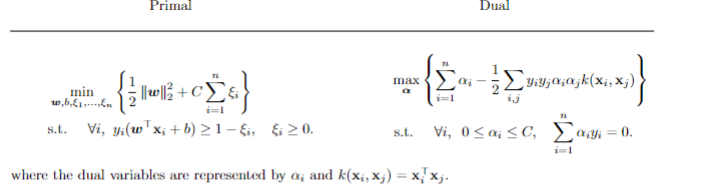
\includegraphics[width=0.8\textwidth]{primal.png}
    \caption{Primal Formulation of SVM}
    \label{fig:primal}
\end{figure}
\newline
[3 points] Find the number of variables to be optimized in the primal and dual forms of SVM. Then, suppose that we decide to use some other kernels (e.g., radial basis kernel, polynomial kernel) instead of the linear kernel \( k(\mathbf{x}_i, \mathbf{x}_j) = \mathbf{x}_i^\top \mathbf{x}_j \). Does this change the number of dual variables we need to use?
\\\\ The primal problem:
\[
\min_{w, b, \xi_1, \ldots, \xi_n} \left( \frac{1}{2} \|w\|_2^2 + C \sum_{i=1}^n \xi_i \right)
\]
Here, we directly optimize \( w \) and \( b \) and introduce slack variables \( \xi_i \) for each data point.


\noindent \textbf{d.} [1 point] Why might you prefer to solve the SVM in the dual formulation as opposed to the primal formulation?
\\\\ The number of variables to be optimized in the primal form of SVM is \( d + 1 \) where \( d \) is the number of features. The number of variables to be optimized in the dual form of SVM is \( n \) where \( n \) is the number of data points. The number of dual variables does not change when using other kernels. You might prefer to solve the SVM in the dual formulation because the dual formulation can be more computationally efficient when the number of data points is larger than the number of features.\\
\newpage
\section {Implementing SVMs}

In this problem, you will experiment with SVMs on a real-world dataset. You will implement a linear SVM (i.e., an SVM using the original features). You should implement it from scratch without using any libraries like scikit-learn, although you can use existing packages to solve quadratic programs. If you are not sure if the library you want to use is allowed, please ask the TAs or post a question on Piazza. We provide you with a guided Python Notebook (hw2\_svm\_imp.ipynb) on which you will find parts you need to fill in. You can use this notebook on JupyterLab / JupyterNotebook / GoogleColab.

Please append your notebook file as a PDF at the end of your submission so that your code and cell outputs can be seen on the same submission PDF. If you use JupyterLab / JupyterNotebook / GoogleColab, you can save the notebook as PDF from File→Print. You can also use online ‘ipynb to pdf’ file converters. Please do not forget to append your notebook as a PDF to the end of your submission PDF for us to grade this question.

Dataset: We have provided the Heart Disease dataset from UCI’s machine learning data repository. The provided binary classification dataset has 13 input features, and 303 samples.

\begin{itemize}
    \item By running the first cell of the given notebook, you download the ucimlrepo package. It will help us download the dataset. For this step, you should have an internet connection.
    \item In the second cell, we provide all required libraries to complete the homework.
    \item In the third cell, we download the dataset (again, you need an internet connection), one-hot encode some categorical features, and split it into train/test parts using a set seed.
\end{itemize}

You should run those three cells without any modification. After running the first three cells, you should have \texttt{X\_train} (shape of (216, 22)), \texttt{X\_test} (shape of (83, 22)), \texttt{y\_train} (shape of (216, )), and \texttt{y\_test} (shape of (83, )) variables.

\begin{enumerate}
    \item  Let $x^{(1)}_k, \cdots, x^{(N)}_k$ be the values of feature $k$ for all training set ($X_{\text{train}}$) points where $N$ is the number of samples in the training set. Preprocess the training ($X_{\text{train}}$) and test data ($X_{\text{test}}$) by:
    \begin{enumerate}
        \item Computing the mean $\bar{x}_k = \frac{1}{N} \sum_{i=1}^{N} x^{(i)}_k$ of each feature and subtracting it from all values of this feature.
        \item Dividing each feature by its standard deviation, defined as
        \[
        s_k = \sqrt{\frac{1}{N} \sum_{i=1}^{N} (x^{(i)}_k - \bar{x}_k)^2}
        \]
        for feature $k$. Here, $\bar{x}_k$ is the sample mean of this feature.
    \end{enumerate}
    Save the normalized data samples as variables named \texttt{X\_train\_normalized} for the training set and \texttt{X\_test\_normalized} for the test set. Note that the shape of these variables should be the same as the shapes of \texttt{X\_train} and \texttt{X\_test}, respectively.

    This type of preprocessing is useful for SVMs, as SVMs attempt to maximize the distance between the separating hyperplane and the support vectors. If one feature (i.e., one dimension in this space) has very large values, it will dominate the other features when calculating this distance. Rescaling the features will ensure that they all have the same influence on the distance metric.

    Note that the mean and standard deviation should be estimated from the training data (\texttt{X\_train}) and then applied to both datasets. This is because using the statistics from the training data ensures that the model is not biased by the test data, which should remain unseen during training.

    Report the mean and the standard deviation of the first and the last features computed on the training data (\texttt{X\_train}):
    \begin{itemize}
        \item Mean of the first feature: $\bar{x}_1$
        \item Standard deviation of the first feature: $s_1$
        \item Mean of the last feature: $\bar{x}_{22}$
        \item Standard deviation of the last feature: $s_{22}$
    \end{itemize}
\end{enumerate}


\end{document}